


%🍁% \chapter{Variables, expressions and statements  |  变量、表达式和语句}
\chapter{变量、表达式和语句}

%🍁% One of the most powerful features of a programming language is the
%🍁% ability to manipulate {\bf variables}.  A variable is a name that
%🍁% refers to a value.

编程语言最强大的特性之一,是操作变量的能力。 {\em 变量}是指向某个值的名称。
\index{variable}  \index{变量}

% \section{Assignment statements  |  赋值语句}
\section{赋值语句}
\label{variables}
\index{assignment statement}  \index{statement!assignment}
\index{赋值语句}  \index{语句!赋值}

%🍁% An {\bf assignment statement} creates a new variable and gives
%🍁% it a value:

{\em 赋值语句} (assignment statement) 可用于新建变量,并为该变量赋值。

\begin{lstlisting}
>>> message = 'And now for something completely different'
>>> n = 17
>>> pi = 3.141592653589793
\end{lstlisting}
%
%🍁% This example makes three assignments.  The first assigns a string
%🍁% to a new variable named {\tt message};
%🍁% the second gives the integer {\tt 17} to {\tt n}; the third
%🍁% assigns the (approximate) value of $\pi$ to {\tt pi}.

这个例子进行了三次赋值。 第一句将一个字符串赋给了名为 \li{message} 的新变量; 第二句将整型数 \li{17} 赋给变量 \li{n}; 第三句将 $\pi$ 的(近似)值赋给变量 \li{pi}。
\index{state diagram}  \index{diagram!state}

%🍁% A common way to represent variables on paper is to write the name with
%🍁% an arrow pointing to its value.  This kind of figure is
%🍁% called a {\bf state diagram} because it shows what state each of the
%🍁% variables is in (think of it as the variable's state of mind).
%🍁% Figure~\ref{fig.state2} shows the result of the previous example.

书面上更常用的表示变量的方法是写下变量名,并用箭头指向变量的值。 这种图被称为状态图 (state diagram) ,因为它展示了每个变量所处的状态(可以把其看成是变量的心理状态)。 图~\ref{fig.state2} 展示了前面例子的结果。

\begin{figure}
\centerline
{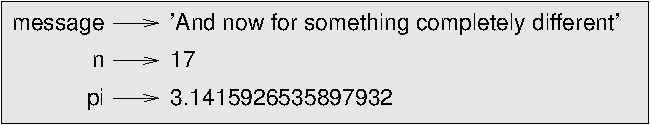
\includegraphics[scale=0.8]{../source/figs/state2.pdf}}
\caption{State diagram.  |  状态图。}
\label{fig.state2}
\end{figure}

% \section{Variable names  |  变量名}
\section{变量名}
\index{variable}
\index{变量}

%🍁% Programmers generally choose names for their variables that
%🍁% are meaningful---they document what the variable is used for.
%🍁%
%🍁% Variable names can be as long as you like.  They can contain
%🍁% both letters and numbers, but they can't begin with a number.
%🍁% It is legal to use uppercase letters, but it is conventional
%🍁% to use only lower case for variables names.
%🍁%
%🍁% The underscore character, \verb"_", can appear in a name.
%🍁% It is often used in names with multiple words, such as
%🍁% \verb"your_name" or \verb"airspeed_of_unladen_swallow".
%🍁% \index{underscore character}
%🍁%
%🍁% If you give a variable an illegal name, you get a syntax error:

程序员通常为变量选择有意义的名字 --- 用于记录变量的用途。

变量名长度可以任意, 它们可以包括字母和数字,但是不能以数字开头。 使用大写字母是合法的, 但是根据惯例, 变量名只使用小写字母。

下划线 (\li{_}) 可以出现在变量名中。 它经常用于有多个单词的变量名,例如 \li{my_name} 或者 \li{airspeed_of_unladen_swallow}。
\index{underscore character} \index{下划线}

如果你给了变量一个非法的名称,解释器将抛出一个语法错误:

\begin{lstlisting}
>>> 76trombones = 'big parade'
SyntaxError: invalid syntax
>>> more@ = 1000000
SyntaxError: invalid syntax
>>> class = 'Advanced Theoretical Zymurgy'
SyntaxError: invalid syntax
\end{lstlisting}

%
%🍁% {\tt 76trombones} is illegal because it begins with a number.
%🍁% {\tt more@} is illegal because it contains an illegal character, {\tt
%🍁% @}.  But what's wrong with {\tt class}?
%🍁%
%🍁% It turns out that {\tt class} is one of Python's {\bf keywords}.  The
%🍁% interpreter uses keywords to recognize the structure of the program,
%🍁% and they cannot be used as variable names.
%🍁% \index{keyword}
%🍁%
%🍁% Python 3 has these keywords:

\li{76trombones} 是非法的,因为它以数字开头。 \li{more@} 因为包含了一个非法字符\li{@}也是非法的。 但是,\li{class} 错在哪儿了呢?

原来,\li{class} 是 Python 的 {\em 关键字} (keywords)之一。 解释器使用关键字识别程序的结构,它们不能被用作变量名。

Python 3有以下关键词:


\begin{lstlisting}
False      class      finally    is         return
None       continue   for        lambda     try
True       def        from       nonlocal   while
and        del        global     not        with
as         elif       if         or         yield
assert     else       import     pass
break      except     in         raise
\end{lstlisting}

%
%🍁% You don't have to memorize this list.  In most development environments,
%🍁% keywords are displayed in a different color; if you try to use one
%🍁% as a variable name, you'll know.

你没有必要熟记这些关键词。 大部分的开发环境会区分颜色显示关键词;如果你不小心使用关键词作为变量名,你会发现的。


% \section{Expressions and statements  |  表达式和语句}
\section{表达式和语句}

%🍁% An {\bf expression} is a combination of values, variables, and operators.
%🍁% A value all by itself is considered an expression, and so is
%🍁% a variable, so the following are all legal expressions:

{\em 表达式} (expression) 是值、变量和运算符的组合。 值和变量自身也是表达式,因此下面的表达式都是合法的:
\index{expression}  \index{表达式}

\begin{lstlisting}
>>> 42
42
>>> n
17
>>> n + 25
42
\end{lstlisting}

%
%🍁% When you type an expression at the prompt, the interpreter
%🍁% {\bf evaluates} it, which means that it finds the value of
%🍁% the expression.
%🍁% In this example, {\tt n} has the value 17 and
%🍁% {\tt n + 25} has the value 42.
%🍁% \index{evaluate}
%🍁%
%🍁% A {\bf statement} is a unit of code that has an effect, like
%🍁% creating a variable or displaying a value.
%🍁% \index{statement}

当你在提示符后输入表达式时,解释器会 {\em 计算} (evaluate) 该表达式,这就意味着解释器会求它的值。在上面的例子中,\li{n} 的值是 \li{17,n + 25} 的值是 \li{42}。
\index{evaluate}

{\em 语句} (statement) 是一个会产生影响的代码单元,例如新建一个变量或显示某个值。
\index{statement}

\begin{lstlisting}
>>> n = 17
>>> print(n)
\end{lstlisting}

%
%🍁% The first line is an assignment statement that gives a value to
%🍁% {\tt n}.  The second line is a print statement that displays the
%🍁% value of {\tt n}.
%🍁%
%🍁% When you type a statement, the interpreter {\bf executes} it,
%🍁% which means that it does whatever the statement says.  In general,
%🍁% statements don't have values.
%🍁% \index{execute}

第一行是一个赋值语句,将某个值赋给了 \li{n}。第二行是一个打印语句,在屏幕上显示 \li{n} 的值。

当你输入一个语句后,解释器会 {\em 执行} (execute) 这个语句,即按照语句的指令完成操作。一般来说,语句是没有值的。
\index{execute}

% \section{Script mode  |  脚本模式}
\section{脚本模式}

%🍁% So far we have run Python in {\bf interactive mode}, which
%🍁% means that you interact directly with the interpreter.
%🍁% Interactive mode is a good way to get started,
%🍁% but if you are working with more than a few lines of code, it can be
%🍁% clumsy.

到目前为止,我们都是在{\em 交互模式} (interactive mode) 下运行 Python,即直接与解释器进行交互。交互模式对学习入门很有帮助,但是如果你需要编写很多行代码,使用交互模式就不太方便了。

%🍁% The alternative is to save code in a file called a {\bf script} and
%🍁% then run the interpreter in {\bf script mode} to execute the script.  By
%🍁% convention, Python scripts have names that end with {\tt .py}.
%🍁% \index{script}  \index{script mode}

另一种方法是将代码保存到一个被称为脚本 (script) 的文件里,然后以脚本模式 (script mode) 运行解释器并执行脚本。按照惯例,Python脚本文件名的后缀是 \li{.py}。
\index{script}  \index{script mode}
\index{脚本}  \index{脚本模式}

%🍁% If you know how to create and run a script on your computer, you
%🍁% are ready to go.  Otherwise I recommend using PythonAnywhere again.
%🍁% I have posted instructions for running in script mode at
%🍁% \url{http://tinyurl.com/thinkpython2e}.

如果你知道如何在本地电脑新建并运行脚本,那你可以开始编码了。否则的话,我再次建议使用\hyperref[python_anywhere]{PythonAnywhere}。我在 \href{http://tinyurl.com/thinkpython2e}{http://tinyurl.com/thinkpython2e} 上贴出了如何以脚本模式运行解释器的指南。

%🍁% Because Python provides both modes,
%🍁% you can test bits of code in interactive mode before you put them
%🍁% in a script.  But there are differences between interactive mode
%🍁% and script mode that can be confusing.
%🍁% \index{interactive mode}  \index{script mode}

由于Python支持这两种模式,在将代码写入脚本之前,你可以在交互模式下对代码片段进行测试。不过,交互模式和脚本模式之间存在一些差异,可能会让你感到疑惑。
\index{interactive mode}  \index{script mode}
\index{交互模式}  \index{脚本模式}

%🍁% For example, if you are using Python as a calculator, you might type

举个例子,如果你把Python当计算器使用,你可能会输入下面这样的代码:

\begin{lstlisting}
>>> miles = 26.2
>>> miles * 1.61
42.182
\end{lstlisting}

%🍁% The first line assigns a value to {\tt miles}, but it has no visible
%🍁% effect.  The second line is an expression, so the
%🍁% interpreter evaluates it and displays the result.  It turns out that a
%🍁% marathon is about 42 kilometers.

第一行将一个值赋给 \li{miles},但是并没有产生可见的效果。 第二行是一个表达式,因此解释器计算它并将结果显示出来。 结果告诉我们,一段马拉松大概是 \li{42} 公里。

%🍁% But if you type the same code into a script and run it, you get no
%🍁% output at all.  In script mode an expression, all by itself, has no
%🍁% visible effect.  Python actually evaluates the expression, but it doesn't
%🍁% display the value unless you tell it to:

但是如果你将相同的代码键入一个脚本并且运行它,你得不到任何输出。 在脚本模式下,表达式自身不会产生可见的效果。虽然Python实际上计算了表达式,但是如果你不告诉它要显示结果,它是不会那么做的。

\begin{lstlisting}
miles = 26.2
print(miles * 1.61)
\end{lstlisting}

%🍁% This behavior can be confusing at first.
%🍁%
%🍁% A script usually contains a sequence of statements.  If there
%🍁% is more than one statement, the results appear one at a time
%🍁% as the statements execute.
%🍁%
%🍁% For example, the script

这个行为开始可能有些令人费解。

一个脚本通常包括一系列语句。 如果有多于一条的语句,那么随着语句逐个执行,解释器会逐一显示计算结果。

例如,以下脚本

\begin{lstlisting}
print(1)
x = 2
print(x)
\end{lstlisting}

%
produces the output

产生的输出结果是

\begin{lstlisting}
1
2
\end{lstlisting}

%
%🍁% The assignment statement produces no output.

%🍁% To check your understanding, type the following statements in the
%🍁% Python interpreter and see what they do:

赋值语句不产生输出。

在Python解释器中键入以下的语句,看看他们的结果是否符合你的理解:

\begin{lstlisting}
5
x = 5
x + 1
\end{lstlisting}

%🍁% Now put the same statements in a script and run it.  What
%🍁% is the output?  Modify the script by transforming each
%🍁% expression into a print statement and then run it again.

现在将同样的语句写入一个脚本中并执行它。输出结果是什么? 修改脚本,将每个表达式变成打印语句,再次运行它。

% \section{Order of operations  |  运算顺序}
\section{运算顺序}
\index{order of operations}  \index{PEMDAS}
\index{运算顺序}

%🍁% When an expression contains more than one operator, the order of
%🍁% evaluation depends on the {\bf order of operations}.  For
%🍁% mathematical operators, Python follows mathematical convention.
%🍁% The acronym {\bf PEMDAS} is a useful way to
%🍁% remember the rules:

当一个表达式中有多于一个运算符时,计算的顺序由 {\em 运算顺序} (order of operations) 决定。 对于算数运算符,Python遵循数学里的惯例。 缩写\textbf{PEMDAS}有助于帮助大家记住这些规则:

%🍁% \begin{itemize}
%🍁%
%🍁% \item {\bf P}arentheses have the highest precedence and can be used
%🍁% to force an expression to evaluate in the order you want. Since
%🍁% expressions in parentheses are evaluated first, {\tt 2 * (3-1)} is 4,
%🍁% and {\tt (1+1)**(5-2)} is 8. You can also use parentheses to make an
%🍁% expression easier to read, as in {\tt (minute * 100) / 60}, even
%🍁% if it doesn't change the result.
%🍁%
%🍁% \item {\bf E}xponentiation has the next highest precedence, so
%🍁% {\tt 1 + 2**3} is 9, not 27, and {\tt 2 * 3**2} is 18, not 36.
%🍁%
%🍁% \item {\bf M}ultiplication and {\bf D}ivision have higher precedence
%🍁%   than {\bf A}ddition and {\bf S}ubtraction.  So {\tt 2*3-1} is 5, not
%🍁%   4, and {\tt 6+4/2} is 8, not 5.
%🍁%
%🍁% \item Operators with the same precedence are evaluated from left to
%🍁%   right (except exponentiation).  So in the expression {\tt degrees /
%🍁%     2 * pi}, the division happens first and the result is multiplied
%🍁%   by {\tt pi}.  To divide by $2 \pi$, you can use parentheses or write
%🍁%   {\tt degrees / 2 / pi}.
%🍁%
%🍁% \end{itemize}

\begin{itemize}

\item {\em 括号} ({\bf P}arentheses) 具有最高的优先级,并且可以强制表达式按你希望的顺序计算。 因为在括号中的表达式首先被计算,那么 \li{2 * (3-1)} 的结果是 \li{4},\li{(1+1)**(5-2)} 的结果是 \li{8}。 你也可以用括号提高表达式的可读性,如写成 \li{(minute * 100) / 60},即使这样并不改变运算的结果。

\item {\em 指数运算} ({\bf E}xponentiation) 具有次高的优先级,因此 \li{1 + 2**3} 的结果是 \li{9} 而非 \li{27}, \li{2 * 3**2} 的结果是 \li{18} 而非 \li{36}。

\item {\em 乘法} ({\bf M}ultiplication) 和 {\em 除法} ({\bf D}ivision) 有相同的优先级, 比 {\em 加法} ({\bf A}ddition) 和 {\em 减法} ({\bf S}ubtraction) 高,加法和减法也具有相同的优先级。 因此 \li{2*3-1} 是 \li{5} 而非 \li{4}, \li{6+4/2} 是 \li{8} 而非 \li{5}。

\item 具有相同优先级的运算符按照从左到右的顺序进行计算(除了指数运算)。 因此表达式 \li{degrees / 2 * pi} 中,除法先运算,然后结果被乘以 \li{pi}。 为了被 $2\pi$ 除,你可以使用括号,或者写成 \li{degrees / 2 / pi}。

\end{itemize}

%🍁% I don't work very hard to remember the precedence of
%🍁% operators.  If I can't tell by looking at the expression, I use
%🍁% parentheses to make it obvious.

我不会费力去记住这些运算符的优先级规则。如果看完表达式后分不出优先级,我会使用括号使计算顺序变得更明显。


%
% \section{String operations  |  字符串运算}
\section{字符串运算}
\index{string!operation}  \index{operator!string}
\index{字符串!操作}  \index{操作!字符串}

%🍁% In general, you can't perform mathematical operations on strings, even
%🍁% if the strings look like numbers, so the following are illegal:

一般来讲,你不能对字符串执行数学运算,即使字符串看起来很像数字, 因此下面这些表达式是非法的:


\begin{lstlisting}
'2'-'1'    'eggs'/'easy'    'third'*'a charm'
\end{lstlisting}

%
%🍁% But there are two exceptions, {\tt +} and {\tt *}.
%🍁%
%🍁% The {\tt +} operator performs {\bf string concatenation}, which means
%🍁% it joins the strings by linking them end-to-end.  For example:

但有两个例外,\li{+} 和 \li{*}。

加号运算符 \li{+} 可用于 字符串拼接 \footnote{string concatenation},也就是将字符串首尾相连起来。例如:
\index{concatenation}

\begin{lstlisting}
>>> first = 'throat'
>>> second = 'warbler'
>>> first + second
throatwarbler
\end{lstlisting}

%
%🍁% The {\tt *} operator also works on strings; it performs repetition.
%🍁% For example, \verb"'Spam'*3" is \verb"'SpamSpamSpam'".  If one of the
%🍁% values is a string, the other has to be an integer.
%🍁%
%🍁% This use of {\tt +} and {\tt *} makes sense by
%🍁% analogy with addition and multiplication.  Just as {\tt 4*3} is
%🍁% equivalent to {\tt 4+4+4}, we expect \verb"'Spam'*3" to be the same as
%🍁% \verb"'Spam'+'Spam'+'Spam'", and it is.  On the other hand, there is a
%🍁% significant way in which string concatenation and repetition are
%🍁% different from integer addition and multiplication.
%🍁% Can you think of a property that addition has
%🍁% that string concatenation does not?
%🍁% \index{commutativity}

乘法运算符 \li{*} 也可应用于字符串;它执行重复运算。 例如,\li{'Spam'*3} 的结果是 \li{'SpamSpamSpam'}。  如果其中一个运算数是字符串,则另外一个必须是整型数。

\li{+} 和 \li{*} 的这个用法,类比加法和乘法也讲得通。 就像 \li{4*3} 与 \li{4+4+4} 等价一样, 我们也会期望 \li{'Spam'*3} 和 \li{'Spam'+'Spam'+'Spam'} 等价,而事实确实如此。 另外,字符串拼接和重复与整数的加法和乘法也有很大的不同。 你能想出来一个加法具有而字符串拼接不具有的特性么?
\index{commutativity}

% \section{Comments  |  注释}
\section{注释}
\index{comment}  \index{注释}

%🍁% As programs get bigger and more complicated, they get more difficult
%🍁% to read.  Formal languages are dense, and it is often difficult to
%🍁% look at a piece of code and figure out what it is doing, or why.
%🍁%
%🍁% For this reason, it is a good idea to add notes to your programs to explain
%🍁% in natural language what the program is doing.  These notes are called
%🍁% {\bf comments}, and they start with the \verb"#" symbol:

随着程序变得越写越长,越来越复杂,它们的可读性也越来越差。 形式语言是稠密的,通常很难在读一段代码后,说出其做什么或者为什么这样做。

因此,在你的程序中需要用自然语言做些笔记,解释程序将做些什么。 这些笔记被称为{\em 注释} (comments),以 \li{#} 符号开始。

\begin{lstlisting}
# compute the percentage of the hour that has elapsed
# 计算逝去的时间占一小时的比例
percentage = (minute * 100) / 60
\end{lstlisting}

%
%🍁% In this case, the comment appears on a line by itself.  You can also put
%🍁% comments at the end of a line:

此例中,注释独占一行。 你也可以将注释放在行尾:

\begin{lstlisting}
percentage = (minute * 100) / 60     # percentage of an hour
\end{lstlisting}

%
%🍁% Everything from the {\tt \#} to the end of the line is ignored---it
%🍁% has no effect on the execution of the program.

从 \li{#} 开始到行尾的所有内容都会被解释器忽略 — 其内容对程序执行不会有任何影响。

%🍁% Comments are most useful when they document non-obvious features of
%🍁% the code.  It is reasonable to assume that the reader can figure out
%🍁% {\em what} the code does; it is more useful to explain {\em why}.

在注释中记录代码不明显的特征,是最有帮助的。 假设读者能够读懂代码做了{\bf 什么}是合理的; 但是解释代码\textbf{为什么}这么做则更有用。

%🍁% This comment is redundant with the code and useless:

下面这个注释只是重复了代码,没有什么用:

\begin{lstlisting}
v = 5     # assign 5 to v
\end{lstlisting}

%
%🍁% This comment contains useful information that is not in the code:

下面的注释包括了代码中没有的有用信息:

\begin{lstlisting}
v = 5     # velocity in meters/second.
\end{lstlisting}

%
%🍁% Good variable names can reduce the need for comments, but
%🍁% long names can make complex expressions hard to read, so there is
%🍁% a tradeoff.

好的变量名能够减少对注释的需求,但是长变量名使得表达式很难读, 因此这里有个平衡问题。

%
% \section{Debugging  |  调试}
\section{调试}
\index{debugging}  \index{bug}
\index{调试}  \index{故障}

%🍁% Three kinds of errors can occur in a program: syntax errors, runtime
%🍁% errors, and semantic errors.  It is useful
%🍁% to distinguish between them in order to track them down more quickly.

程序中可能会出现下面三种错误:{\em 语法错误} (syntax error)、 {\em 运行时错误} (runtime error) 和 {\em 语义错误} (semantic error)。 区别三者的差异有助于快速追踪这些错误。

%🍁% \begin{description}
%🍁%
%🍁% \item[Syntax error:] ``Syntax'' refers to the structure of a program
%🍁%   and the rules about that structure.  For example, parentheses have
%🍁%   to come in matching pairs, so {\tt (1 + 2)} is legal, but {\tt 8)}
%🍁%   is a {\bf syntax error}.  \index{syntax error} \index{error!syntax}
%🍁%   \index{error message}
%🍁% \index{syntax}
%🍁%
%🍁% If there is a syntax error
%🍁% anywhere in your program, Python displays an error message and quits,
%🍁% and you will not be able to run the program.  During the first few
%🍁% weeks of your programming career, you might spend a lot of
%🍁% time tracking down syntax errors.  As you gain experience, you will
%🍁% make fewer errors and find them faster.
%🍁%
%🍁%
%🍁% \item[Runtime error:] The second type of error is a runtime error, so
%🍁%   called because the error does not appear until after the program has
%🍁%   started running.  These errors are also called {\bf exceptions}
%🍁%   because they usually indicate that something exceptional (and bad)
%🍁%   has happened.  \index{runtime error} \index{error!runtime}
%🍁%   \index{exception} \index{safe language} \index{language!safe}
%🍁%
%🍁% Runtime errors are rare in the simple programs you will see in the
%🍁% first few chapters, so it might be a while before you encounter one.
%🍁%
%🍁%
%🍁% \item[Semantic error:] The third type of error is ``semantic'', which
%🍁%   means related to meaning.  If there is a semantic error in your
%🍁%   program, it will run without generating error messages, but it will
%🍁%   not do the right thing.  It will do something else.  Specifically,
%🍁%   it will do what you told it to do.  \index{semantic error}
%🍁%   \index{error!semantic} \index{error message}
%🍁%
%🍁% Identifying semantic errors can be tricky because it requires you to work
%🍁% backward by looking at the output of the program and trying to figure
%🍁% out what it is doing.
%🍁%
%🍁% \end{description}

\begin{description}

\item[语法错误:] 语法指的是程序的结构及其背后的规则。 例如, 括号必须要成对出现, 所以 \li{(1 + 2)} 是合法的, 但是 \li{8)} 则是一个 语法错误。
\index{syntax}  \index{语法}

如果你的程序中存在一个语法错误,Python会显示一条错误信息,然后退出运行。你无法顺利运行程序。在你编程生涯的头几周里,你可能会花大量时间追踪语法错误。随着你的经验不断积累,犯的语法错误会越来越少,发现错误的速度也会更快。


\item[运行时错误:] 第二种错误类型是运行时错误,这么称呼是因为这类错误只有在程序开始运行后才会出现。这类错误也被称为 {\em 异常} (exception) ,因为它们的出现通常说明发生了某些特别的(而且不好的)事情。
  \index{runtime error} \index{error!runtime}
  \index{exception} \index{safe language} \index{language!safe}
  \index{运行时错误} \index{错误!运行时}
  \index{异常} \index{safe language} \index{language!safe}

在前几章提供的简单程序中,你很少会碰到运行时错误,所以你可能需要一段时间才会接触到这种错误。


\item[语义错误:] 第三类错误是“语义”错误,即与程序的意思的有关。如果你的程序中有语义错误,程序在运行时不会产生错误信息,但是不会返回正确的结果。它会返回另外的结果。严格来说,它是按照你的指令在运行。
  \index{semantic error}  \index{error!semantic}  \index{error message}
  \index{语义错误}  \index{错误!语义}  \index{错误信息}
识别语义错误可能是棘手的,因为这需要你反过来思考,通过观察程序的输出来搞清楚它在做什么。

\end{description}


% \section{Glossary  |  术语表}
\section{术语表}

%🍁% \begin{description}
%🍁%
%🍁% \item[variable:]  A name that refers to a value.
%🍁% \index{variable}
%🍁%
%🍁% \item[assignment:]  A statement that assigns a value to a variable.
%🍁% \index{assignment}
%🍁%
%🍁% \item[state diagram:]  A graphical representation of a set of variables and the
%🍁% values they refer to.
%🍁% \index{state diagram}
%🍁%
%🍁% \item[keyword:]  A reserved word that is used to parse a
%🍁% program; you cannot use keywords like {\tt if}, {\tt  def}, and {\tt while} as
%🍁% variable names.
%🍁% \index{keyword}
%🍁%
%🍁% \item[operand:]  One of the values on which an operator operates.
%🍁% \index{operand}
%🍁%
%🍁% \item[expression:]  A combination of variables, operators, and values that
%🍁% represents a single result.
%🍁% \index{expression}
%🍁%
%🍁% \item[evaluate:]  To simplify an expression by performing the operations
%🍁% in order to yield a single value.
%🍁%
%🍁% \item[statement:]  A section of code that represents a command or action.  So
%🍁% far, the statements we have seen are assignments and print statements.
%🍁% \index{statement}
%🍁%
%🍁% \item[execute:]  To run a statement and do what it says.
%🍁% \index{execute}
%🍁%
%🍁% \item[interactive mode:] A way of using the Python interpreter by
%🍁% typing code at the prompt.
%🍁% \index{interactive mode}
%🍁%
%🍁% \item[script mode:] A way of using the Python interpreter to read
%🍁% code from a script and run it.
%🍁% \index{script mode}
%🍁%
%🍁% \item[script:] A program stored in a file.
%🍁% \index{script}
%🍁%
%🍁% \item[order of operations:]  Rules governing the order in which
%🍁% expressions involving multiple operators and operands are evaluated.
%🍁% \index{order of operations}
%🍁%
%🍁% \item[concatenate:]  To join two operands end-to-end.
%🍁% \index{concatenation}
%🍁%
%🍁% \item[comment:]  Information in a program that is meant for other
%🍁% programmers (or anyone reading the source code) and has no effect on the
%🍁% execution of the program.
%🍁% \index{comment}
%🍁%
%🍁% \item[syntax error:]  An error in a program that makes it impossible
%🍁% to parse (and therefore impossible to interpret).
%🍁% \index{syntax error}
%🍁%
%🍁% \item[exception:]  An error that is detected while the program is running.
%🍁% \index{exception}
%🍁%
%🍁% \item[semantics:]  The meaning of a program.
%🍁% \index{semantics}
%🍁%
%🍁% \item[semantic error:]   An error in a program that makes it do something
%🍁% other than what the programmer intended.
%🍁% \index{semantic error}
%🍁%
%🍁% \end{description}

\begin{description}

\item[变量 (variable):]  变量是指向某个值的名称。
\index{variable}  \index{变量}

\item[赋值语句 (assignment):]  将某个值赋给变量的语句。
\index{assignment}  \index{赋值语句}

\item[状态图 (state diagram):]  变量及其所指的值的图形化表示。
\index{state diagram}  \index{状态图}

\item[关键字 (keyword):]  关键字是用于解析程序的;你不能使用if、def和while这样的关键词作为变量名。
\index{keyword}  \index{关键字}

\item[运算数 (operand):]  运算符所操作的值之一。
\index{operand}  \index{运算数}

\item[表达式 (expression):]  变量、运算符和值的组合,代表一个单一的结果。
\index{expression}  \index{表达式}

\item[计算 (evaluate):]  通过执行运算以简化表达式,从而得出一个单一的值。

\item[语句 (statement):]  代表一个命令或行为的一段代码。 目前为止我们接触的语句有赋值语句和打印语句。
\index{statement}  \index{语句}

\item[执行 (execute):]  运行一个语句,并按照语句的指令操作。
\index{execute}  \index{执行}

\item[交互式模式 (interactive mode):]  通过在提示符中输入代码,使用Python解释器的一种方式。
\index{interactive mode}  \index{交互式模式}

\item[脚本模式 (script mode):]  使用Python解释器从脚本中读取代码,并运行脚本的方式。
\index{script mode}  \index{脚本模式}

\item[脚本 (script):]  保存在文件中的程序。
\index{script}  \index{脚本}

\item[运算顺序 (order of operations):]  有关多个运算符和运算数时计算顺序的规则。
\index{order of operations}  \index{运算顺序}

\item[拼接 (concatenate):]  将两个运算数首尾相连。
\index{concatenation}  \index{拼接}

\item[注释 (comment):]  程序中提供给其他程序员(任何阅读源代码的人)阅读的信息,对程序的执行没有影响。
\index{comment}  \index{注释}

\item[语法错误 (syntax error):]  使得程序无法进行解析(因此无法进行解释)的错误。
\index{syntax error}  \index{语法错误}

\item[异常 (exception):]  只有在程序运行时才发现的错误。
\index{exception}  \index{异常}

\item[语义 (semantics):]  程序中表达的意思。
\index{semantics}  \index{语义}

\item[语义错误 (semantic error):]  使得程序偏离程序员原本期望的错误。
\index{semantic error}  \index{语义错误}

\end{description}


% \section{Exercises  |  练习}
\section{练习}

\begin{exercise}

%🍁% Repeating my advice from the previous chapter, whenever you learn
%🍁% a new feature, you should try it out in interactive mode and make
%🍁% errors on purpose to see what goes wrong.

%🍁% \begin{itemize}

%🍁% \item We've seen that {\tt n = 42} is legal.  What about {\tt 42 = n}?

%🍁% \item How about {\tt x = y = 1}?

%🍁% \item In some languages every statement ends with a semi-colon, {\tt ;}.
%🍁% What happens if you put a semi-colon at the end of a Python statement?

%🍁% \item What if you put a period at the end of a statement?

%🍁% \item In math notation you can multiply $x$ and $y$ like this: $x y$.
%🍁% What happens if you try that in Python?

%🍁% \end{itemize}

和上一章一样,我还是要建议大家在学习新特性之后,在交互模式下充分试验,故意犯一些错误,看看到底会出什么问题。

\begin{itemize}

\item 我们已经知道 {\em \li{n = 42}} 是合法的。那么 {\em \li{42 = n}} 呢?

\item {\em \li{x = y = 1}} 合法吗?

\item 在某些编程语言中,每个语句都是以分号 {\em \li{;}} 结束的。如果你在一个{\em Python}语句后也以分号结尾,会发生什么?

\item 如果在语句最后带上分号呢?

\item 在数学记法中,你可以将  $x$ 和  $y$ 像这样相乘: $x y$ 。如果你在 {\em Python} 中也这么写的话,会发生什么?

\end{itemize}

\end{exercise}


%
%%
\begin{exercise}

%🍁% Practice using the Python interpreter as a calculator:
%🍁% \index{calculator}

%🍁% \begin{enumerate}
%🍁%
%🍁% \item The volume of a sphere with radius $r$ is $\frac{4}{3} \pi r^3$.
%🍁%   What is the volume of a sphere with radius 5?
%🍁%
%🍁% \item Suppose the cover price of a book is \$24.95, but bookstores get a
%🍁%   40\% discount.  Shipping costs \$3 for the first copy and 75 cents
%🍁%   for each additional copy.  What is the total wholesale cost for
%🍁%   60 copies?
%🍁%
%🍁% \item If I leave my house at 6:52 am and run 1 mile at an easy pace
%🍁%   (8:15 per mile), then 3 miles at tempo (7:12 per mile) and 1 mile at
%🍁%   easy pace again, what time do I get home for breakfast?
%🍁% \index{running pace}
%🍁%
%🍁% \end{enumerate}

继续练习将 {\em Python} 解释器当做计算器使用:
\index{计算器}

\begin{enumerate}

\item 半径为 $r$ 的球体积是 $\frac{4}{3} \pi r^3$ 。 半径为 $5$ 的球体积是多少?

\item 假设一本书的零售价是 {\em \$24.95},但书店有 {\em 40\%} 的折扣。运费则是第一本 {\em \$3} ,以后每本 {\em 75} 美分。 购买 {\em 60} 本的总价是多少?

\item 如果我上午 {\em 6:52} 离开家, 以轻松跑 {\em (easy pace)}的速度跑 {\em 1} 里(即每英里耗时{\em 8}分{\em 15}秒), 再以节奏跑 {\em (tempo)} 的速度跑 {\em 3} 英里(每英里耗时{\em 7}分{\em 12}秒), 之后又以放松跑的速度跑 {\em 1} 英里, 我什么时候回到家吃早饭? \footnote{译者注:配速(pace)是在马拉松运动的训练中常使用的一个概念,配速是速度的一种,是每公里所需要的时间。配速=时间/距离。Tempo run 一般被翻译成「节奏跑」或「乳酸门槛跑」,是指以比10K或5K比赛速度稍慢(每公里大约慢10--15秒)的速度进行训练,或者以平时15K-半程的配速来跑。参考:https://www.zhihu.com/question/22237002}
\index{running pace}

\end{enumerate}

\end{exercise}